% Messwerte: Alle gemessenen Größen tabellarisch darstellen
% Auswertung: Berechnung geforderter Ergebnisse mit Schritten/Fehlerformeln/Erläuterung/Grafik (Programme)
\section{Auswertung}
\label{sec:auswertung}

\begin{figure}[H]
	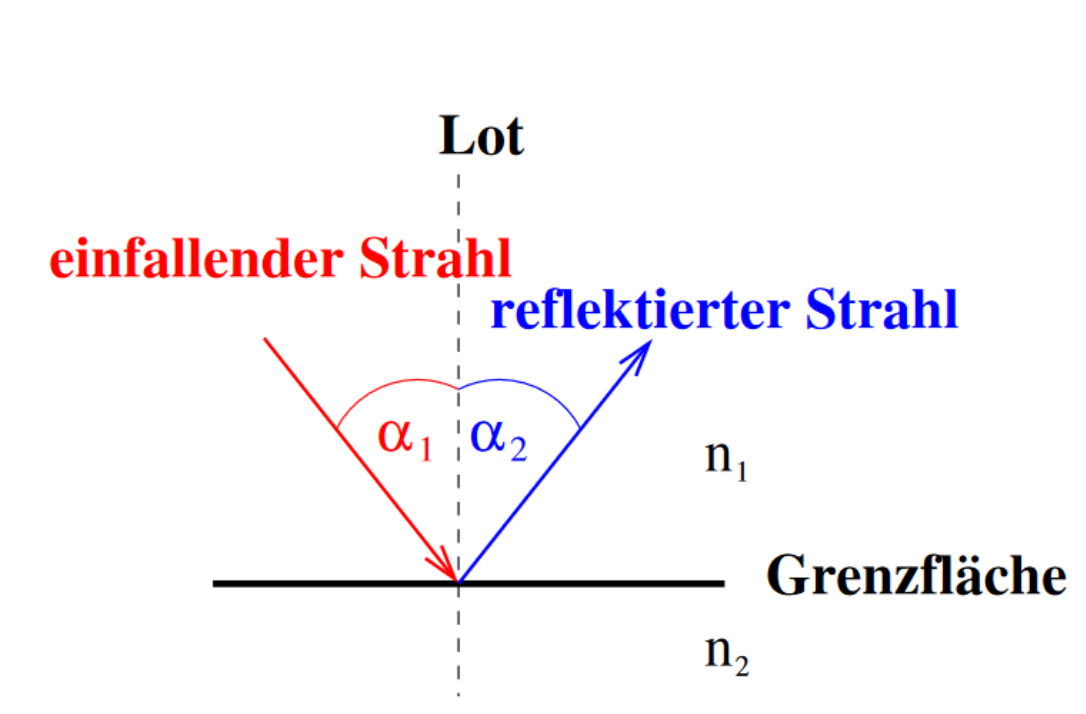
\includegraphics{build/reflexion.pdf}
	\caption{}
	\label{fig:reflexion}
\end{figure}

\begin{figure}[H]
	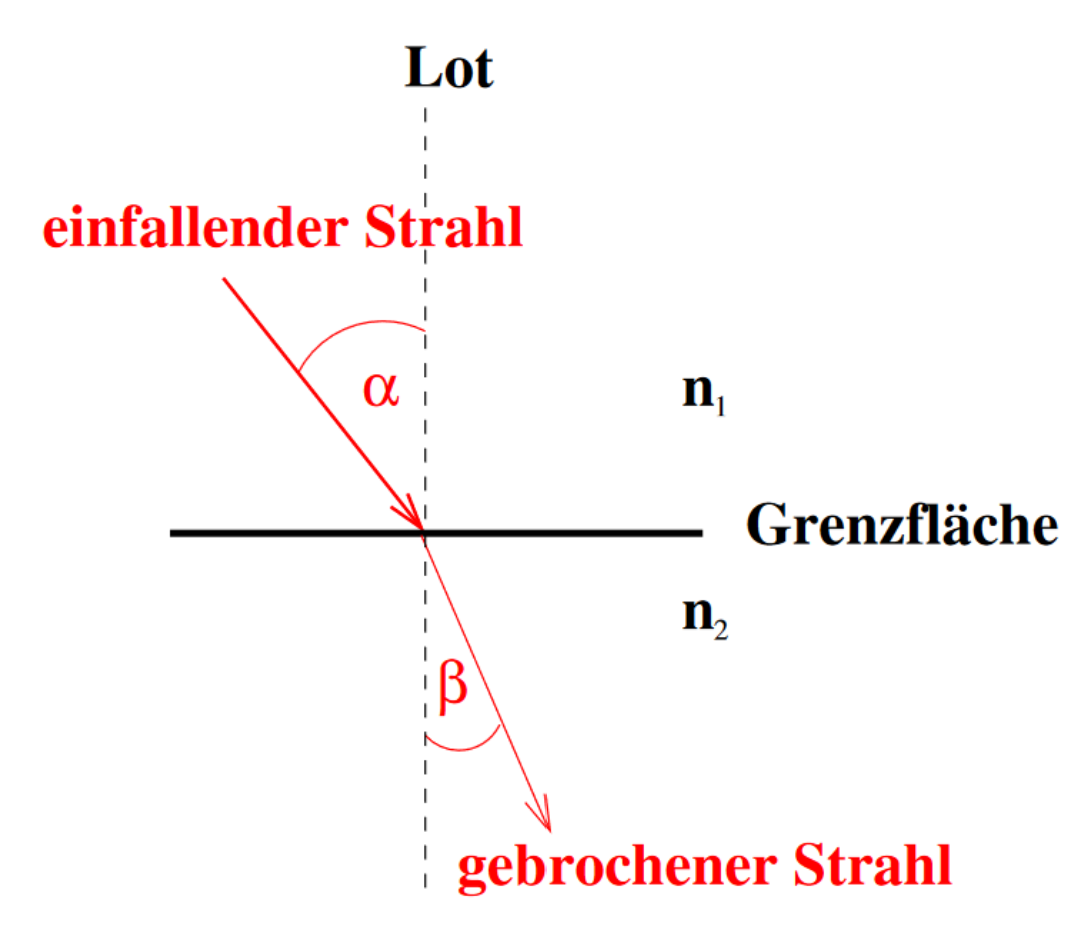
\includegraphics{build/brechung.pdf}
	\caption{}
	\label{fig:brechung}
\end{figure}

\begin{figure}[H]
	\includegraphics{build/beugung.pdf}
	\caption{}
	\label{fig:beugung}
\end{figure}
